%%%%%%%%%%%%%%%%%%%%%%% file template.tex %%%%%%%%%%%%%%%%%%%%%%%%%
%
% This is a general template file for the LaTeX package SVJour3
% for Springer journals.          Springer Heidelberg 2010/09/16
%
% Copy it to a new file with a new name and use it as the basis
% for your article. Delete % signs as needed.
%
% This template includes a few options for different layouts and
% content for various journals. Please consult a previous issue of
% your journal as needed.
%
%%%%%%%%%%%%%%%%%%%%%%%%%%%%%%%%%%%%%%%%%%%%%%%%%%%%%%%%%%%%%%%%%%%
%
% First comes an example EPS file -- just ignore it and
% proceed on the \documentclass line
% your LaTeX will extract the file if required
\begin{filecontents*}{example.eps}
%!PS-Adobe-3.0 EPSF-3.0
%%BoundingBox: 19 19 221 221
%%CreationDate: Mon Sep 29 1997
%%Creator: programmed by hand (JK)
%%EndComments
gsave
newpath
  20 20 moveto
  20 220 lineto
  220 220 lineto
  220 20 lineto
closepath
2 setlinewidth
gsave
  .4 setgray fill
grestore
stroke
grestore
\end{filecontents*}
%
\RequirePackage{fix-cm}
%
%\documentclass{svjour3}                     % onecolumn (standard format)
%\documentclass[smallcondensed]{svjour3}     % onecolumn (ditto)
\documentclass[smallextended]{svjour3}       % onecolumn (second format)
%\documentclass[twocolumn]{svjour3}          % twocolumn
%
\smartqed  % flush right qed marks, e.g. at end of proof
%
\usepackage{graphicx}
\usepackage{amsmath}
\usepackage{amssymb}
\usepackage{natbib}
\usepackage{bm}
\usepackage{amsfonts}
\usepackage{amsmath}
\usepackage{amssymb}
\usepackage{algorithm}
\usepackage{algorithmic}




\DeclareMathOperator*{\argmin}{arg\,min}
\DeclareMathOperator*{\argmax}{arg\,max}
\DeclareMathOperator\E{\mathbb{E}}
\DeclareMathOperator\Var{\mathrm{Var}}
\def\R{\mathbb{R}}
\def\P{\mathcal{P}}
\usepackage{mathtools}
\DeclarePairedDelimiter\abs{\lvert}{\rvert}
\DeclarePairedDelimiter\norm{\lVert}{\rVert}
\DeclarePairedDelimiter\inner{\langle}{\rangle}
\DeclarePairedDelimiter\floor{\lfloor}{\rfloor}
\DeclarePairedDelimiter\ceil{\lceil}{\rceil}
\makeatletter
\newcommand{\algorithmicfunction}{\textbf{function}}
\newcommand{\algorithmicendfunction}{\algorithmicend\ \algorithmicfunction}
\newenvironment{ALC@func}{\begin{ALC@g}}{\end{ALC@g}}
\newcommand{\FUNCTION}[2][default]{\ALC@it\algorithmicfunction\ #2\ %
\textbf{:}%
\ALC@com{#1}\begin{ALC@func}}
\ifthenelse{\boolean{ALC@noend}}{
    \newcommand{\ENDFUNCTION}{\end{ALC@func}}
  }{
    \newcommand{\ENDFUNCTION}{\end{ALC@func}\ALC@it\algorithmicendfunction}
  }
\makeatother


%
% \usepackage{mathptmx}      % use Times fonts if available on your TeX system
%
% insert here the call for the packages your document requires
%\usepackage{latexsym}
% etc.
%
% please place your own definitions here and don't use \def but
% \newcommand{}{}
%
% Insert the name of "your journal" with
\journalname{Machine Learning}
%
\begin{document}

\title{Graph-Based Info-Clustering and its Applications%\thanks{Grants or other notes
%about the article that should go on the front page should be
%placed here. General acknowledgments should be placed at the end of the article.}
}
%\subtitle{Do you have a subtitle?\\ If so, write it here}

%\titlerunning{Short form of title}        % if too long for running head

\author{First Author         \and
        Second Author %etc.
}

%\authorrunning{Short form of author list} % if too long for running head

\institute{F. Author \at
              first address \\
              Tel.: +123-45-678910\\
              Fax: +123-45-678910\\
              \email{fauthor@example.com}           %  \\
%             \emph{Present address:} of F. Author  %  if needed
           \and
           S. Author \at
              second address
}

\date{Received: date / Accepted: date}
% The correct dates will be entered by the editor


\maketitle

\begin{abstract}
We propose a graph-based hierarchical clustering method based on a multivariate information metric.
The proposed method can generate non-binary hierarchical tree that reveals the intrinsic structures in the data, with no hyper-parameter to tune. 
The hierarchical tree can be computed efficiently using
our improved algorithm. Besides clustering task, we show that our method can be adopted and
used in outlier detection and community discovery problems.
Experiments show that the clustering result outperforms
other hierarchical clustering techniques and is very suitable to find the complex community structure.
\keywords{First keyword \and Second keyword \and More}
% \PACS{PACS code1 \and PACS code2 \and more}
% \subclass{MSC code1 \and MSC code2 \and more}
\end{abstract}

\section{Introduction}
\label{intro}
% background information goes here
Clustering Analysis is an important research topic in machine learning.
It has wide applications in many areas. For example, to track the epidemic
sources within a community and assist for the model of natural disasters with observed data.

There are many different methods for clustering analysis. One of them is called
hierarchical clustering. The classical method uses the Euclid distance between samples
as the metric to merge the most similar pairs until all the samples are merged into a clustering
tree \citep{slink}. Compared with other clustering method, hierarchical clustering can better describe the relationship between different clusters. Still, the classical hierarchical clustering method has some
drawbacks. One of them is pairwise merging, which is not optimal since it does not consider information shared among more than two clusters. Besides, the criterion to split the clustering tree into a flat clustering structure is arbitrary set and lacks explanations, which bring some mysteries in practical
usage.

In recent 20 years, there are many emerging hierarchical clustering methods which brought new insights into this area. These new methods arise from combination of different domain knowledge and
subject branch. To name but a few, hierarchical density estimation \citep{hde}, Bayesian hierarchical clustering \citep{bhc},
clusterpath based on convex optimization \citep{hocking2011clusterpath},
graph partition based on Dasgupta's cost \citep{dasgupta2016cost},
Gradient-based Hierarchical Clustering based on hyperbolic gemetry \citep{hyperbolic} etc.
These methods have both advantages and disadvantages.
In practice researchers need to choose the proper method according to the specific problem.
For example, an extension called Bayesian Rose Trees of Bayesian clustering
can produce non-binary hierarchical tree
under a given probabilistic model \citep{blundell2011discovering} and have XXX advantages.
But Bayesian model has many hyper-parameters to tune and the clustering results between different runs vary greatly because of its intrinsic randomness.
This method is suitable for problems which XXX.

Besides the hierarchical methods mentioned above, there is a specific branch which brings information theory into clustering. This branch is based on the observation that metrics in hierarchical clusterings
are mostly empirically inspired and may not reflect the true underlining probalistic model of the data.
Either variants of mutual information or some other kind of information-theoretic metric \citep{ic2002}  is used in the past literature. For the former method, the metric of mutual information is used and an agglomerative scheme is adopted \citep{mim}. The mutual information between samples and cluster labels is estimated using Parzen' window, which is a kind of Gaussian mixture model. Such adoption
has some theoretical benefits but suffers from sub-optimization of mutual information cost in the agglomerative approximation. It is until the proposal of multivariate mutual information metric in clustering that there is some breakthrough \citep{ic2016}.

Multivariate mutual information, as its name suggests, is an extension of mutual information for multiple
random variables. Using such metric as the thresholds, \citet{ic2016} shows that we can get a clustering
tree for random variables. The theory sounds good but it is nearly impossible to compute such metric
in practice. Similar issues exist for Bayesian probabilistic approach. For these probablistic methods, we
are unable to estimate precisely the distribution from data. While prametric model is used in Bayesian
method, we will propose a graph model to apply multivariate mutual information for clustering.

Reducing from abstract probablistic space to graph model is not a crazy idea but origins from the local regime assumption of distributions. It's known that estimation of mutual information between $X$ and $Y$ from data is a hard task but when $X$ and $Y$ are nearly indepedent, \citet{huang2017information} shows that the estimation can be simplied to do some kind of alternative conditional expectation, which is much easier
than estimating probabilty distribution function. In this paper, we will extend this local regime result to multivariate case and show how it is equivalent to a graph model.

Many problems in graph model are NP-Hard and only allows approximation solutions. Quite surprisingly, our proposed graph-based clustering method is polynomial-time efficient solvable exactly.
This result has been established by using a special graph partition structure called "Principal Sequence of Partition"(PSP), which is equivalent to our divisive approach. The compution of "Principal Lattice" allows a polynomial time algorithm.
However, the original algorithm proposed by
\citet{narayanan}, which is used directly by \citet{mac}, has a high time complexity to fit the practice. There has been some improvement
using parametric maximal flow techniques \citep{kolmogorov}, which is later adopted for graph model
by \citet{pin}. Though these two improvements share the same time complexity, we will show that our improvement runs almost an order of magnitude faster than the parametric approach under a fair implementation environment.

There has been little prior work on applying Info-Clustering methods to data engineering problems except for some proof-of-concept experiment \citep{mac}. In this paper, we will consider the application
of our graph-based Info-Clustering to different unsupervised learning problems. Specifically
we will not only consider data clustering problems, in which our proposed method can be directly applied, but also for outlier detection and community discovery problems we will propose new promising
method adopted from graph-based Info-Clustering. We will conduct empirical experiments on both artificially generated data and some real-world dataset and show the feasibility of our method in
data engineering problems.

The paper is organized as follows: In Section \ref{sec:bk} we introduce the backgrond knowledge of the theorical Info-Clustering, its relationship with PSP structure and theory of local geometry information. In Section \ref{sec:GBIC} our formulation of graph-based Info-Clustering(GBIC) and important properties of our model are given. In Section \ref{sec:alg}, we propose an improved algorithm to compute the PSP structure of graph. Then in Section \ref{sec:es} we conduction empirical study of GBIC on data clustering, outlier detection and community discovery. Finally we give the conclusion in Section \ref{sec:conc}.


\section{Background Knowledge}\label{sec:bk}
Before proceeding to introduce our theoretical and algorithmic results, it is necessary to review some prior results from minimal technical aspect. We split this section into three parts, first we introduce
the local information geometry theory and the concept of weak dependency of two random variables;
next is the general info-clustering model and its relationship with principal sequence of partitions (PSP) of submodular function;
the final part is about the original algorithm used to solve PSP problem when the submodular function
is graph cut function.
\subsection{Local Information Geometry}
It is well known that KL-Divengence can be used to measure the distance of two probabistic distributions. When the two distributions are quite "near", that is, both of them are within a neighborhood of a distribution $P$, we can simplify the expression of KL-Divergence as the Euclid distance \citep{huang2017information}. To be more specific, we use the example of discrete distribution and use $P_0$ to represent a distribution on alphabet $\mathcal{X}$. We say $P$ is in a $\epsilon$-Neighborhood $N^{(\epsilon)}(P_0)$ of $P_0$ if
\begin{equation}
P \in N^{(\epsilon)}(P_0) \iff \sum_{x \in \mathcal{X}} \frac{(P(x) - P_0(x))^2}{P(x)} < \epsilon^2
\end{equation}
The above equation can be expressed in concise form if we write $P(x) = P_0(x) + \epsilon
\sqrt{P_0(x)} \phi(x)$, in which $\phi(x)$ is treated as feature vector. Then we have $||\phi || < 1$.
If both $P_1, P_2 \in N^{(\epsilon)}(P_0)$ we have
\begin{equation}
D(P_1 || P_2) = \frac{\epsilon^2}{2} ||\phi_1 - \phi_2||^2 + o(\epsilon^2)
\end{equation}
In addition, the above result can be used when two random variables are weakly independent \citep{huang2019universal}. That is, we say $X$ and $Y$ are weakly dependent if the conditional distribution $Y|X(\cdot |x) \in N^{(\epsilon)}(Y)$ for all $x \in \mathcal{X}$. Under the assumption of
weak dependence the mutual information, which is defined by $D(P_{XY}||P_XP_Y)$ can be expressed
in concise form:
\begin{equation}\label{eq:Ixy}
I(X;Y) = \frac{1}{2}\sum_{x\in \mathcal{X}, y\in \mathcal{Y}} B^2(x,y) + o(\epsilon^2) \textrm{ where }  B(x,y)=\frac{P_{X,Y}(x,y) - P_X(x) P_Y(y)}{\sqrt{P_X(x)P_Y(y)}}
\end{equation}
To simplify the notation, the term $\sum_{x\in \mathcal{X}, y\in \mathcal{Y}} B^2(x,y)$ can be regarded as the square of Frobenious norm $\norm{B}_F^2$ for matrix $\bm{B}$. Equation \eqref{eq:Ixy} gives the domaint term
of the mutual information when the random variables are weakly dependent.

\subsection{Theoretical Info-Clustering}
There are many ways to extend mutual information for multiple random variables. \cite{ic2016} gives one based on partition of set $V$. All partitions of $V$ except for $\{V\}$ consists the non-trivial partition collection $\Pi'(V)$ and the multivariate mutual information(MMI) of $\{Z_i | i \in V\}$ is defined as:
\begin{align}
I(Z_V) &:= \min_{P \in \Pi'(V)} I_{P}(Z_V) \textrm{ where} \\
I_P(Z_V) &:= \frac{1}{|P| - 1}D(P_{Z_V} || \prod_{C\in P} P_{Z_C})
\end{align}
Based on the definition of MMI, the cluster can be obtained by considering all maximal subsets $B$ such that $I(Z_B) > \gamma$ for a certain threshold $\gamma$. All such $B$ consists of $\mathcal{C}(Z_V)$.
This is the theoretical definition of clusters, which is equivalent to the algorithmic one:

\begin{equation}\label{eq:CZV}
C(Z_V) = \{ V\} \cup \bigcup_{B \in \mathcal{C}_{\gamma_1}} \mathcal{C}(Z_B) \textrm{ where } \gamma_1 = I(Z_V)
\end{equation}

Equation \eqref{eq:CZV} gives a divisive approach to obtain all clusters and threshold values from
the largest set $V$ and smallest threshold value $\gamma_1$. However, we cannot get a feasible algorithm
to compute the clusters since it is unknown how to compute $I(Z_V)$.
To get over this difficulty a relationship between $I(Z_V)$ and a special kind of submodular function minimization problem is established \citep{mac}: All threshold values and clusters are the same as those of
the following optimization problem with $f[\mathcal{P}]=D(P_{Z_V} || \prod_{C\in P}P_{Z_C})$:
\begin{align}\label{eq:hPLambda}
h_{\mathcal{P}}(\lambda) &= f[\mathcal{P}] - |\mathcal{P}| \lambda \notag\\
h(\lambda) &= \min_{\mathcal{P} \in \Pi'(V)}h_{\mathcal{P}}(\lambda)
\end{align}
In the above equation, $h(\lambda)$ is a piecewise linear function about $\lambda$ with turning points
$\lambda_1, \dots, \lambda_{k}$. The general solution for \eqref{eq:hPLambda} can be written as
\begin{equation}
h(\lambda) = \begin{cases} h_{P_0}(\lambda) & \lambda < \lambda_1 \\
h_{P_i}(\lambda) & \lambda_i \leq \lambda < \lambda_{i+1} \textrm{ for } i = 1, \dots, k-1 \\
h_{P_k}(\lambda) & \lambda \geq \lambda_k
\end{cases}
\end{equation}
Furthermore, we have $P_0 \succeq P_1 \dots \succeq P_k$ \citep{narayanan}. That is, partition $P_{i+1}$ is a refinement of $P_i$.

\subsection{Efficient Algorithm to solve PSP structure}
\cite{narayanan} proposes a divide and conquer approach to solve the PSP structure from equation \eqref{eq:hPLambda} for a general submodular function. Since the optimal partition is $P_0 = \{V\}$ when $\lambda=0$ and the partition is $P_k=\{\{1\}, \{2\}, \dots, \{|V|\}\}$ when $\lambda$ is quite large,
his method starts from two endpoints $\lambda_i = 0, \lambda_j = +\infty$ and find the intersection of 
$h(\lambda_i)$ and $h(\lambda_j)$ at $(\lambda', h')$. Then we compute a partition $P'$ such that $h(\lambda') = h_{P'}(\lambda')$. By definition $h(\lambda') \leq h'$ and when the strict inequality is taken we can repeat the process within $(\lambda_i, \lambda')$ and $(\lambda', \lambda_j)$ respectively. The technique procedure is documented in Algorithm \ref{alg:psp}.
\begin{algorithm}
\caption{PSP algorithm}\label{alg:psp}
\begin{algorithmic}[1]
\REQUIRE Statistics of $Z_V$ sufficient for calculating $f(B)$ for all $B \subseteq V$
\ENSURE A sorted critical value array \textbf{L} and a reverse ordered array \textbf{PSP} containing $\P_1,\dots, P_k$.
\STATE \textbf{L}  $\leftarrow$ empty list.
\STATE $Q\leftarrow \{V\}, P \leftarrow \{ \{i \} | i \in V\}$
\STATE $\mathbf{PSP}= [Q, P]$
\STATE \texttt{Split}$(Q,P)$
\STATE sort $L$ and sort $\mathbf{PSP}$ with respect to $\succeq$ 
\FUNCTION{\texttt{Split}$(Q,P)$}
 \STATE\label{alg:gamma} $\gamma' = {1 \over \abs{P} - \abs{Q}} (f(P)-f(Q))$
 \STATE $h' = {1 \over \abs{P} - \abs{Q}}(\abs{P} f(Q) - \abs{Q} f(P))$
 \STATE $(\tilde{h}, P') = \texttt{DT}(f,\gamma')$ \footnotemark
 \IF{$\tilde{h} = h'$}
 	\STATE insert $\gamma'$ to $\mathbf{L}$
 \ELSE
 	\STATE insert $P'$ to $\mathbf{PSP}$
 	\STATE \texttt{Split}$(Q, P')$
 	\STATE \texttt{Split}$(P',P)$
 \ENDIF
\ENDFUNCTION
\end{algorithmic}
\end{algorithm}

In Algorithm \ref{alg:psp}, a function DT is used to get the miminal value. There are some candicates for this function, throughout this paper we use the one proposed by \cite{mac}. Since the theoretical and algorithmic detail is not correlated with this paper, we omit their introduction.

\section{Formulation of graph-based Info-clustering}\label{sec:GBIC}

General model of Info-Clustering is not very useful since we know little about the joint distribution.
We need to do some kind of model reduction to get some useful model. In particular, it has been shown
by \cite{ic2016} that when $Z_1, \dots, Z_n$ forms a Markov chain, then we can get a model called Mutual Information Relevance Network \citep{butte1999mutual}. In the following section we will show
that the general model reduces to our graph-based Info-Clustering when $Z_1, \dots, Z_n$ are weakly
independent. The relationship of these two special models, together with their parent model, are shown
in the Vienn diagram in Fig. \ref{fig:relationship} % For one-column wide figures use

\begin{figure}
\centering
% Use the relevant command to insert your figure file.
% For example, with the graphicx package use
  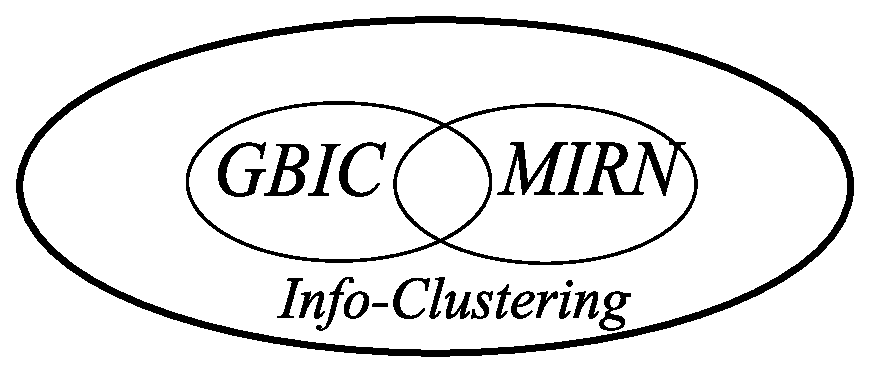
\includegraphics[width=6cm]{relationship.eps}
% figure caption is below the figure
\caption{General Info clustering models reduces to GBIC or MIRN model respectively under different assumptions for the joint distribution}
\label{fig:relationship}       % Give a unique label
\end{figure}

From local geometry information it is known that two random variables $X$ and $Y$ are weakly dependent if
\begin{equation}
P_{Y|X=x}(y) = P_Y(y) +\epsilon \phi_x(y) \sqrt{P_Y(y)}
\end{equation}
where $\norm{\phi_x}\leq 1$.

For multiple random variables we give:

\begin{definition}\label{def:general}
$X_1, \dots, X_n$ are weakly dependent if there exist a random variable $U$ such that
$(X_1, \dots, X_n)$ is weakly dependent with $U$ and $X_1, \dots X_n$ are independent conditioned
on $U$.
\end{definition}

Let $\Pi$ be the partition of $V=\{1,2,\dots, n\}$. We claim:
\begin{theorem}\label{thm:wd_multiple}
If $X_1, \dots, X_n$ are weakly dependent, then
\begin{equation}
D(P_{X_V} || \prod_{C\in \Pi} P_{X_{C}}) = {1 \over 2}\sum_{\substack{(i,j) \not\in C\\ C\in \Pi}} \norm{B_{ij}}_F^2 + o(\epsilon^2)
\end{equation}
\end{theorem}
We can see that Theorem \ref{thm:wd_multiple} is an extension of the approximation of mutual equation in Equation \eqref{eq:Ixy} to the case of multiple random variables.
%
% For two-column wide figures use
% \begin{figure*}
% Use the relevant command to insert your figure file.
% For example, with the graphicx package use
 % \includegraphics[width=0.75\textwidth]{example.eps}
% figure caption is below the figure
% \caption{Please write your figure caption here}
%\label{fig:2}       % Give a unique label
%\end{figure*}
%
\section{Improved PSP Algorithms}\label{sec:alg}
\section{Empirical Study of GBIC}\label{sec:es}
\subsection{Data Clustering Scenario}\label{subsec:dc}
\subsection{Info-Detection for Outlier Detection}\label{subsec:od}
\subsection{Community Detection Field}\label{subsec:cd}
\section{Conclusion}\label{sec:conc}

%\begin{acknowledgements}
%If you'd like to thank anyone, place your comments here
%and remove the percent signs.
%\end{acknowledgements}


% Authors must disclose all relationships or interests that 
% could have direct or potential influence or impart bias on 
% the work: 
%
% \section*{Conflict of interest}
%
% The authors declare that they have no conflict of interest.


% BibTeX users please use one of
\bibliographystyle{spbasic}      % basic style, author-year citations
%\bibliographystyle{spmpsci}      % mathematics and physical sciences
%\bibliographystyle{spphys}       % APS-like style for physics
\bibliography{exportlist.bib}   % name your BibTeX data base

% Non-BibTeX users please use
%\begin{thebibliography}{}
%
% and use \bibitem to create references. Consult the Instructions
% for authors for reference list style.
%
%\bibitem{RefJ}
% Format for Journal Reference
%Author, Article title, Journal, Volume, page numbers (year)
% Format for books
%\bibitem{RefB}
%Author, Book title, page numbers. Publisher, place (year)
% etc
%\end{thebibliography}

\end{document}
% end of file template.tex

